\documentclass[aspectratio=43,9pt]{beamer}
\let\Tiny=\tiny
%
\usepackage{tikz}
\usepackage{enumerate}
%
\usetheme{Boadilla}
%
%
\let\Tiny=\tiny%			% to avoid warnings about font size
%\usepackage{lmodern}%		% alternative method to avoid these warnings
%
\catcode`~=11 % make LaTeX treat tilde (~) like a normal character
\newcommand{\urltilde}{\hbox{~}}
\catcode`~=13 % revert back to treating tilde (~) as an active character
%
% misc commands
\newcommand{\bm}[1]{\mathbf{#1}}
\newcommand{\bs}[1]{\boldsymbol{#1}}
\newenvironment{myitemize}[1]{\vspace{#1}\begin{itemize}\setlength\itemsep{#1}}{\end{itemize}}
%
% pgf markers
\usepgflibrary{plotmarks}
%
\setbeamertemplate{footline}
{
  \leavevmode%
  \hbox{%
  \begin{beamercolorbox}[wd=.8\paperwidth,ht=2.25ex,dp=1ex,left]{author in head/foot}%
    \usebeamerfont{author in head/foot}\hspace*{4em}\inserttitle
  \end{beamercolorbox}%
  \begin{beamercolorbox}[wd=.2\paperwidth,ht=2.25ex,dp=1ex,right]{author in head/foot}%
    \usebeamerfont{author in head/foot}\insertframenumber{} / \inserttotalframenumber\hspace*{1ex}
  \end{beamercolorbox}}%
  \vskip0pt%
}
%
\setbeamertemplate{navigation symbols}{}
%
\setbeamertemplate{frametitle}
{%
	\begin{minipage}{.9\paperwidth}
		\vspace*{1ex}%
		\flushright%
		%\bfseries
		\LARGE%
		\insertframetitle%
	\end{minipage}%
}
%
\setbeamertemplate{title page}{
	\begin{center}
		\vspace*{2ex}
		\usebeamercolor[fg]{frametitle}{%
			\Large%
			Numerical Techniques 2025--2026\\[2ex]
			%
			\LARGE%
			\inserttitle
		}\\[6ex]
		\usebeamercolor[fg]{normal text}{%
			Daan Degrauwe\\[1ex]
			\texttt{daan.degrauwe@meteo.be}\\[4ex]
			Postgraduate Studies in Weather and Climate Modeling\\[1ex]
			Ghent University
		}
	\end{center}
}
%
\newcommand{\ft}[2]{{\textstyle\frac{#1}{#2}}}
%
% increase space around equations
\makeatletter
\g@addto@macro\normalsize{%
	\setlength{\abovedisplayskip}{3ex}%
	\setlength{\belowdisplayskip}{3ex}%
	\setlength{\abovedisplayshortskip}{3ex}%
	\setlength{\belowdisplayshortskip}{3ex}%
}%
\makeatother
%

%
\title{1. Discretization and stability}%
%
%%%%%%%%%%%%%%%%%%%%%%%%%%%%%%%%%%%%%%%%%%%%%%%%%%%%%%%%%%%%%%%%%%%%%%
%
\begin{document}
%
%%%%%%%%%%%%%%%%%%%%%%%%%%%%%%%%%%%%%%%%%%%%%%%%%%%%%%%%%%%%%%%%%%%%%%%%%%%%%%%%%%%%%%%%%%%%%%%%%%%%
%
\begin{frame}[plain]
	\titlepage
\end{frame}
%
%%%%%%%%%%%%%%%%%%%%%%%%%%%%%%%%%%%%%%%%%%%%%%%%%%%%%%%%%%%%%%%%%%%%%%
%
\begin{frame}
	%
	\frametitle{Content}
	%
	%\tableofcontents
	\large
	%
	\begin{itemize}
		\item Discretization\vspace*{1ex}
		\item A prototype system: the 1D advection equation\vspace*{1ex}
		\item An example of a numerical scheme: the upstream scheme\vspace*{1ex}
		\item Accuracy and consistency\vspace*{1ex}
		\item Convergence\vspace*{1ex}
		\item Stability\vspace*{1ex}
	\end{itemize}		
\end{frame}
%
%%%%%%%%%%%%%%%%%%%%%%%%%%%%%%%%%%%%%%%%%%%%%%%%%%%%%%%%%%%%%%%%%%%%%%%%%%%%%%%%%%%%%%%%%%%%%%%%%%%%
%
\begin{frame}
	%
	\frametitle{Discretization}
	%
	\begin{itemize}
		\item Meteorological fields (temperature, wind, pressure, humidity, \ldots) are continuous in time and space.
		\item On a computer you cannot represent a continuous field; you would need an infinity of points.
		\item So a field will be \emph{discretized}, i.e. it is represented by the values in a set of discrete points:\\[2mm]
			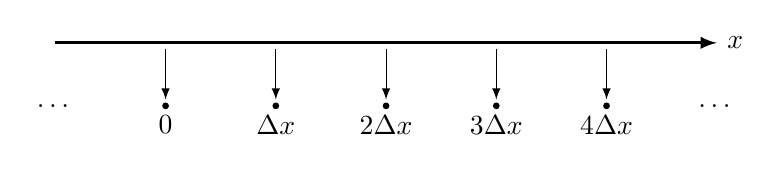
\begin{tikzpicture}[>=latex,x=1.4cm,y=.8cm]
				\draw[line width=1pt,->] (0,1) -- (6,1) node[right] {$x$};
				\draw[->] (1,0) +(0,.9) -- +(0,.1);
				\draw[->] (2,0) +(0,.9) -- +(0,.1);
				\draw[->] (3,0) +(0,.9) -- +(0,.1);
				\draw[->] (4,0) +(0,.9) -- +(0,.1);
				\draw[->] (5,0) +(0,.9) -- +(0,.1);
				\draw[fill] (0,0) node {\ldots}
					(1,0) circle (1pt) node[below] {$0$}
					(2,0) circle (1pt) node[below] {$\Delta x$}
					(3,0) circle (1pt) node[below] {$2\Delta x$}
					(4,0) circle (1pt) node[below] {$3\Delta x$}
					(5,0) circle (1pt) node[below] {$4\Delta x$}
					(6,0) node {\ldots};
			\end{tikzpicture}\\[2mm]
			replacing the continuous coordinate $x$ by discrete points $i \Delta x$ labeled by $i$. Note that $i$ is variable, and $\Delta x$ is constant!
		\item 
			similarly in 2D: $i \Delta x, j \Delta y$
		\item discretizing time: $n \Delta t$
	\end{itemize}
\end{frame}
%
%%%%%%%%%%%%%%%%%%%%%%%%%%%%%%%%%%%%%%%%%%%%%%%%%%%%%%%%%%%%%%%%%%%%%%
%
\begin{frame}
	%
	\frametitle{Discretization of derivatives: finite differences}
	%
	\begin{itemize}
			%
		\item Many physical laws are differential equations\vspace*{2ex}
			%
		\item Some definition of the derivative in $x$:
			\begin{align*}
				\frac{df}{dx} (x_0) &= \lim_{\delta x \rightarrow 0}%
					\frac{f(x_0+\delta x) - f(x_0)}{\delta x}
				\\
				\frac{df}{dx} (x_0) &= \lim_{\delta x \rightarrow 0}%
					\frac{f(x_0) - f(x_0-\delta x)}{\delta x}
				\\
				\frac{df}{dx} (x_0) &= \lim_{\delta x \rightarrow 0}%
					\frac{f(x_0+\delta x) - f(x_0 - \delta x)}{2 \delta x}
				\end{align*}\vspace*{2ex}
			%
		\item On our discrete grid we can't take the limit $\delta x \rightarrow 0$, so the derivative is computed with a finite value $\delta x \rightarrow \Delta x$ (i.e. the grid distance).
			%
	\end{itemize}
	%
\end{frame}
%
%%%%%%%%%%%%%%%%%%%%%%%%%%%%%%%%%%%%%%%%%%%%%%%%%%%%%%%%%%%%%%%%%%%%%%
%
\begin{frame}
	%
	\frametitle{Discretization of derivatives: finite differences}
	%
	\begin{itemize}
		\item The limit is then better approximated by increasing the resolution
			%
			\begin{center}
				%
				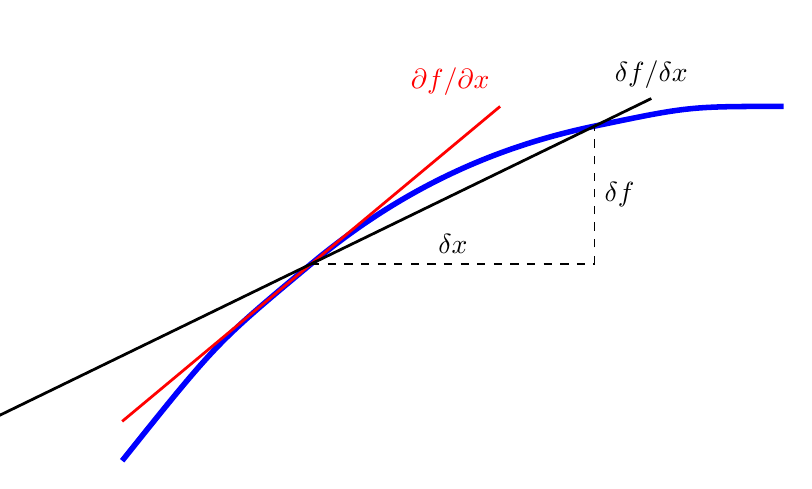
\begin{tikzpicture}[y=5mm,x=12mm]
					\useasboundingbox (-3,-5) -- (5,6);
					\draw [blue, line width=2pt] (-2,-5) .. controls (-1,-2) .. (0,0) .. controls (1,2) and (2,3) .. (3,3.5) .. controls (4,4) .. (5,4);
					\draw [red,line width=1pt] (-2,-4) -- (2,4) node[red,above left] {$\partial f/\partial x$};
					\draw [black,line width=1pt] (-3.6,-4.2) -- (3.6,4.2) node[black,above] {$\delta f/\delta x$};
					\draw [dashed, line width=.5pt] (0,0) -- (3,0) node[pos=.5,black,above] {$\delta x$};
					\draw [dashed, line width=.5pt] (3,0) -- (3,3.5) node[pos=.5,black,right] {$\delta f$};
				\end{tikzpicture}
				%
			\end{center}
			%
	\end{itemize}
	%
\end{frame}
%
%%%%%%%%%%%%%%%%%%%%%%%%%%%%%%%%%%%%%%%%%%%%%%%%%%%%%%%%%%%%%%%%%%%%%%
%
\begin{frame}
	%
	\frametitle{The 1D advection equation}
	%
	We will now consider the 1D advection equation with constant advection\vspace*{3ex}
	%
	\begin{equation*}
		\frac{\partial \psi}{\partial t} + c \frac{\partial \psi}{\partial x} = 0
	\end{equation*}\vspace*{3ex}
	%
	Why?
	%
	\begin{itemize}
		\item hyperbolic systems can be decomposed into decoupled equations of this type\vspace*{1ex}
		\item most systems studied with atmospheric models are hyperbolic.
	\end{itemize}
	%
\end{frame}
%
%%%%%%%%%%%%%%%%%%%%%%%%%%%%%%%%%%%%%%%%%%%%%%%%%%%%%%%%%%%%%%%%%%%%%%
%
\begin{frame}
	%
	\frametitle{The 1D advection equation}
	%
	Physical interpretation of the advection equation:
	%
	\begin{itemize}
		\item $\psi$ is any (meteorological) field: temperature, pressure, humidity, pollutant concentration, \ldots
		\item $c$ is the wind speed.
		\item time evolution: the field is \emph{transported} with speed $c$:
	\end{itemize}\vspace*{2ex}
	%
	\begin{center}
		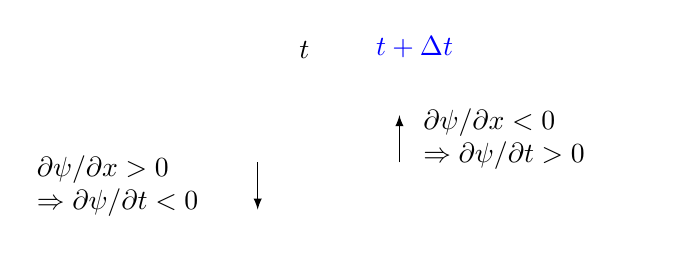
\begin{tikzpicture}[x=6mm,y=6mm,>=latex]
			\draw[black] plot file {figures/nt1/y1.dat};
			\draw (5,5) node[above left,black] {$t$};
			\draw[->] (3.7,3) -- (3.7,2);
			\draw (3.4,2.5) node[left] {\parbox{25mm}{$\partial \psi/\partial x > 0$\\$\Rightarrow \partial \psi/\partial t <0$}};
			\draw[->] (6.7,3) -- (6.7,4);
			\draw (7,3.5) node[right] {\parbox{30mm}{$\partial \psi/\partial x < 0$\\$\Rightarrow \partial \psi/\partial t >0$}};
		\uncover<2->{
			\draw[blue] plot file {figures/nt1/y2.dat};
			\draw (6,5) node[above right,blue] {$t+\Delta t$};
		}
		\end{tikzpicture}
	\end{center}
\end{frame}
%
%%%%%%%%%%%%%%%%%%%%%%%%%%%%%%%%%%%%%%%%%%%%%%%%%%%%%%%%%%%%%%%%%%%%%%
%
\begin{frame}
	%
	\frametitle{The 1D advection equation}
	%
	The exact solution of the advection equation\vspace*{2ex}
	%
	\begin{equation*}
		\frac{\partial \psi}{\partial t}+c\frac{\partial\psi}{\partial x}=0
	\end{equation*}\vspace*{2ex}
	%
	is given by\vspace*{2ex}
	%
	\begin{equation*}
		\psi(x,t) = \psi(x-ct,t=0)
	\end{equation*}
	%
\end{frame}
%
%%%%%%%%%%%%%%%%%%%%%%%%%%%%%%%%%%%%%%%%%%%%%%%%%%%%%%%%%%%%%%%%%%%%%%
%
\begin{frame}
	%
	\frametitle{The upstream scheme}
	%
	Let us call $\phi_j^n$ the solution of the discretized system at time $n \Delta t$ and at grid point $j \Delta x$.\vspace*{2ex}
	%
	\par
	We replace the derivatives by,\vspace*{2ex}
	%
	\begin{align*}
		\frac{\partial \psi}{\partial t} &\rightarrow \frac{\phi_j^{n+1} - \phi_j^n}{\Delta t}\\
		\frac{\partial \psi}{\partial x} &\rightarrow  \frac{\phi_j^n - \phi_{j-1}^n}{\Delta x}
	\end{align*}\par\vspace*{2ex}
	%
	in the advection equation:\vspace*{2ex}
	%
	\begin{equation*}
		\frac{\phi_j^{n+1} - \phi_j^n}{\Delta t}
		+ c \frac{\phi_j^n - \phi_{j-1}^n}{\Delta x} = 0
	\end{equation*}\par\vspace*{2ex}
	%
	This is called the \emph{upstream scheme}.
\end{frame}
%
%%%%%%%%%%%%%%%%%%%%%%%%%%%%%%%%%%%%%%%%%%%%%%%%%%%%%%%%%%%%%%%%%%%%%%
%
\begin{frame}
	%
	\frametitle{The upstream scheme}
	%
	This equation can be solved w.r.t. $\phi_j^{n+1}$:\vspace*{2ex}
	%
	\begin{equation*}
		\phi_j^{n+1} = (1-\mu) \phi_j^n + \mu \phi_{j-1}^n
	\end{equation*}\par\vspace*{2ex}
	%
	with $\mu = c \Delta t / \Delta x$.
	%
	\par\vspace*{2ex}
	So if the solution is known at time $t=n\Delta t$,\\ then it can be calculated at $t=(n+1)\Delta t$.
	%
\end{frame}
%
%%%%%%%%%%%%%%%%%%%%%%%%%%%%%%%%%%%%%%%%%%%%%%%%%%%%%%%%%%%%%%%%%%%%%%
%
\begin{frame}
	\frametitle{The upstream scheme}
	%
	\begin{itemize}
		\item But we see that increasing the spatial resolution doesn't necessarily improve the solution !?\vspace*{2ex}
			%
			\par
			We say that the discretized system becomes \emph{unstable}.\vspace*{3ex}
		\item Stability is a central concept in this course. This lesson will (try to) explain why.\vspace*{2ex}
		\item For this we need additional concepts: accuracy, consistency and convergence.
	\end{itemize}
	%
\end{frame}
%
%%%%%%%%%%%%%%%%%%%%%%%%%%%%%%%%%%%%%%%%%%%%%%%%%%%%%%%%%%%%%%%%%%%%%%
%
\begin{frame}
	%
	\frametitle{Accuracy}
	%
	%
	Using a Taylor expansion\vspace*{2ex}
	%
	\begin{equation*}
		f(x_0+\Delta x) = f(x_0) +
		\Delta x \frac{df}{dx} (x_0)
		+ \frac{\Delta x^2}{2} \frac{d^2f}{dx^2} (x_0)
		+ \frac{\Delta x^3}{6} \frac{d^3 f}{dx^3} (x_0) + \dots
	\end{equation*}\par\vspace*{2ex}
	%
	the error in the approximation of the derivative is\vspace*{2ex}
	%
	\begin{equation*}
		\frac{f(x_0+\Delta x) - f(x_0)}{\Delta x}
		- \frac{d f}{dx} (x_0) =
		\frac{\textcolor{green!60!black}{\Delta x}}{2} \frac{d^2 f}{dx^2} (x_0)
		+ \frac{\Delta x^2}{6} \frac{d^3 f}{dx^3} (x_0) + \dots
	\end{equation*}\par\vspace*{2ex}
	%
	The leading term is proportional to $\Delta x$, so this is called a first-order accurate method.\vspace*{2ex}
	%
\pause
	\par
	Considering the centered finite-difference approximation
	\begin{equation*}
		\frac{f(x_0+\Delta x) - f(x_0 - \Delta x)}{2 \Delta x}
		- \frac{d f}{dx} (x_0) =
		\frac{\textcolor{green!60!black}{\Delta x^2}}{6} \frac{d^3 f}{dx^3} (x_0) +
		\frac{\Delta x^4}{120} \frac{d^5 f}{dx^5} (x_0) + \dots
	\end{equation*}\par\vspace*{2ex}
	%
	we see that it is second-order accurate.
	%
\end{frame}
%
%%%%%%%%%%%%%%%%%%%%%%%%%%%%%%%%%%%%%%%%%%%%%%%%%%%%%%%%%%%%%%%%%%%%%%
%
\begin{frame}
	%
	\frametitle{Higher-order accuracy}
	%
	By using more information (more gridpoints), it is possible to obtain a more accurate approximation for the derivative:\vspace*{3ex}
	%
	\begin{align*}
		\frac{df}{dx} (x_0) = &
		\frac43 \left(
			\frac{f(x_0 + \Delta x) - f(x_0 - \Delta x)}{2 \Delta x}
		\right)\\
		&-\frac13 \left(
			\frac{f(x_0 + 2\Delta x) - f(x_0 - 2 \Delta x)}{4 \Delta x}
		\right)
		+ O[\Delta x^4 ]
	\end{align*}
	%
\end{frame}
%
%%%%%%%%%%%%%%%%%%%%%%%%%%%%%%%%%%%%%%%%%%%%%%%%%%%%%%%%%%%%%%%%%%%%%%
%
\begin{frame}
	%
	\frametitle{Consistency}
	%
	A scheme is called \emph{consistent} if the truncation error converges to zero when $\Delta x \rightarrow 0$ and $\Delta t \rightarrow 0$.
	%
	\par\vspace*{3ex}
	For example, the truncation error for the upstream scheme is:\vspace*{2ex}
	%
	\begin{equation*}
		\frac{\psi_j^{n+1} - \psi_j^n}{\Delta t}
		+ c \frac{\psi_j^n - \psi_{j-1}^n}{\Delta x} = 
		\frac{\Delta t}{2} \frac{\partial^2 \psi}{\partial t^2}
		- c \frac{\Delta x}{2} \frac{\partial^2 \psi}{\partial x^2} + \dots
	\end{equation*}\par\vspace*{2ex}
	%
	where $\psi$ denotes the exact solution.
	%
\end{frame}
%
%%%%%%%%%%%%%%%%%%%%%%%%%%%%%%%%%%%%%%%%%%%%%%%%%%%%%%%%%%%%%%%%%%%%%%
%
\begin{frame}
	%
	\frametitle{Convergence}
	%
	A finite-difference scheme is called \emph{convergent} of order $(p,q)$\\ if in the limit $\Delta t, \Delta x \rightarrow 0$, the numerical solution $\phi_j^n$ satisfies\vspace*{4ex}
	%
	\begin{equation*}
	\| \psi (n \Delta t, j \Delta x ) - \phi_j^n \| = O [ \Delta t^p ] + O [ \Delta x^q ]
	\end{equation*}
	%
\end{frame}
%
%%%%%%%%%%%%%%%%%%%%%%%%%%%%%%%%%%%%%%%%%%%%%%%%%%%%%%%%%%%%%%%%%%%%%%
%
\begin{frame}
	%
	\frametitle{Convergence vs. consistence}
	%
	Consistency tells you something about the equations, convergence tells you about the solution.
	%
	\par\vspace*{3ex}
	The upstream scheme example shows that these two are not identical: it is consistent but not convergent.
	%
	\par\vspace*{3ex}
	There's a problem with the usability of convergence: it relies on the exact solution, which is unknown in most cases.
	%
\end{frame}
%
%%%%%%%%%%%%%%%%%%%%%%%%%%%%%%%%%%%%%%%%%%%%%%%%%%%%%%%%%%%%%%%%%%%%%%
%
\begin{frame}
	%
	\frametitle{Lax theorem}
	%
	The Lax equivalence theorem says that:\\
	%
	\begin{center}
		\bfseries
		If a finite-difference scheme is {linear}, {stable}, and {consistent},\\
		then it is {convergent}
	\end{center}
	%
\pause
	\par\vspace*{4ex}
	Importance: \parbox[t]{.6\textwidth}{in practice we never know the true solution, but we can check if the scheme is \emph{consistent} and \emph{stable}.}
	%
	\par\vspace*{3ex}
	But when is a scheme stable?
	%
\end{frame}
%
%%%%%%%%%%%%%%%%%%%%%%%%%%%%%%%%%%%%%%%%%%%%%%%%%%%%%%%%%%%%%%%%%%%%%%
%
\begin{frame}
	%
	\frametitle{Numerical stability}
	%
	A sufficient condition for stability is that\vspace*{2ex}
	%
	\begin{equation*}
		\| \phi^n \| \le \| \phi^0 \| \quad \text{for all timesteps} \quad n>0
	\end{equation*}\par\vspace*{5ex}
	%
	Again, we don't need to know the true solution for this!
	%
\end{frame}
%
%%%%%%%%%%%%%%%%%%%%%%%%%%%%%%%%%%%%%%%%%%%%%%%%%%%%%%%%%%%%%%%%%%%%%%
%
\begin{frame}
	%
	\frametitle{Checking stability}
	%
	\begin{itemize}
		\item It is difficult to check the evolution of $\| \phi^n \|$ in general.\vspace*{2ex}
			%
		\item Von Neumann proposed to check stability by considering harmonic functions:
			%
			\begin{equation*}
				\phi(x)=\exp(ik x)=\cos(kx)+i\sin(kx)
			\end{equation*}
			%
			\begin{center}
				\bfseries
				If a scheme is stable for all harmonic functions (i.e. all values of $k$),\\ then it is also stable for all (non-harmonic) functions.
			\end{center}\vspace*{2ex}
			%
		\item Because harmonic functions are eigenfunctions of the differential operator, one can express their time evolution as a multiplication with an \emph{amplification factor} $A_k$:
			%
			\begin{equation*}
				\phi^{n}=A_k\phi^{n-1}=\left(A_k\right)^n\phi^0
			\end{equation*}\par\vspace*{2ex}
			%
		\item So stability requires $\|A_k\|\leq 1$, for all $k$.
			%
	\end{itemize}
	%
\end{frame}
%
%%%%%%%%%%%%%%%%%%%%%%%%%%%%%%%%%%%%%%%%%%%%%%%%%%%%%%%%%%%%%%%%%%%%%%
%
\begin{frame}
	%
	\frametitle{Example: stability of the upstream scheme}
	%
	Let us consider again the upstream scheme for the advection equation:
	%
	\begin{equation*}
		\phi_j^{n+1} = (1-\mu) \phi_j^n + \mu \phi_{j-1}^n
	\end{equation*}
	%
	with $\mu = c \Delta t / \Delta x$.
	%
	\par\vspace*{6ex}
	\textbf{What is the amplification factor?}
	%
\pause
	\par\vspace*{4ex}
	First, assume that $\phi_j^n=(A_k)^ne^{ikj\Delta x}$, so\vspace*{2ex}
	%
	\begin{equation*}
		(A_k)^{n+1} e^{ik j \Delta x} = (A_k)^{n}(1-\mu )e^{ikj \Delta x}
		+ (A_k)^{n}\mu e^{ik(j-1) \Delta x}
	\end{equation*}
	%
\pause
	The amplification factor $A_k$ then becomes
	%
	\begin{align*}
		A_k &= 1 -\mu +\mu e^{-ik \Delta x}	\\
			&=(1-\mu+\mu\cos k\Delta x) - i \mu\sin k\Delta x
	\end{align*}
	%
\end{frame}
%
%%%%%%%%%%%%%%%%%%%%%%%%%%%%%%%%%%%%%%%%%%%%%%%%%%%%%%%%%%%%%%%%%%%%%%
%
\begin{frame}
	%
	\frametitle{Example: stability of the upstream scheme}
	%
	\textbf{Is the amplification factor smaller than 1?}
	%
\pause
\par\vspace*{2ex}
	The modulus of the complex number $A_k$ is given by
	%
	\begin{equation*}
		| A_k |^2 = 1 - 2 \mu \left( 1 -\mu \right) \left( 1 - \cos k \Delta x \right)
	\end{equation*}
	%
\pause
	\par\vspace*{2ex}
	This will be $\le 1$ for all values of $k$ if
	%
	\begin{equation*}
		\mu \left( 1 - \mu \right) \ge 0
	\end{equation*}
	%
	i.e. if
	%
	\begin{equation*}
		0 \le \frac{c \Delta t }{\Delta x} \le 1
	\end{equation*}
	%
\end{frame}
%
%%%%%%%%%%%%%%%%%%%%%%%%%%%%%%%%%%%%%%%%%%%%%%%%%%%%%%%%%%%%%%%%%%%%%%
%
\begin{frame}
	%
	\frametitle{Example: stability of the upstream scheme}
	%
	\begin{itemize}
		\item So the upstream scheme is \emph{conditionally stable}, i.e. stability depends on the values of $c$, $\Delta x$ and $\Delta t$.\\[4ex]
		\item In general,
			%
			\begin{itemize}
				\item higher spatial resolution is less stable
				\item smaller timesteps is more stable
				\item higher velocity is less stable\\[4ex]
			\end{itemize}
		\item $\mu=\frac{c \Delta t }{\Delta x}$ is called the Courant number.\\[4ex]
		\item The condition $\mu\leq 1$ is called the Courant-Fredrichs-Lewy (CFL) criterion.
	\end{itemize}
	%
\end{frame}
%
%%%%%%%%%%%%%%%%%%%%%%%%%%%%%%%%%%%%%%%%%%%%%%%%%%%%%%%%%%%%%%%%%%%%%%
%
\begin{frame}
	%
	\frametitle{Workflow}
	%
	Starting from a discretized equation:\vspace*{2ex}
	%
	\begin{enumerate}
		\item Check if the scheme is linear and consistent\vspace*{1ex}
		\item Fill in a harmonic solution $\phi_j^n=(A_k)^n e^{i\,kj\Delta x}$ in the discretized equation\vspace*{1ex}
		\item Calculate (the modulus of) the amplification factor $A_k$\vspace*{1ex}
		\item If $|A_k| \leq 1$, the scheme is stable\vspace*{1ex}
		\item If the scheme is stable and consistent, it is convergent\vspace*{1ex}
		\item If the scheme is convergent, the \emph{error on the solution} can be reduced by increasing the resolution
	\end{enumerate}
	%
\end{frame}
%
%%%%%%%%%%%%%%%%%%%%%%%%%%%%%%%%%%%%%%%%%%%%%%%%%%%%%%%%%%%%%%%%%%%%%%
%
\begin{frame}
	%
	\frametitle{Summary}
	%
	\begin{itemize}
		\item \emph{Discretization} of a continuous function on a grid\vspace*{2ex}
		\item Approximation of derivatives with \emph{finite differences}\vspace*{2ex}
		\item \emph{Accuracy} and \emph{Consistency} of a scheme (error on equations)\vspace*{2ex}
		\item \emph{Convergence} of a scheme (error on solution)\vspace*{2ex}
		\item \emph{Stability} of a scheme: Von Neumann analysis, Courant number and CFL criterion\vspace*{2ex}
		\item Applied to the upstream scheme to solve the 1D advection equation
	\end{itemize}
\end{frame}
%
%%%%%%%%%%%%%%%%%%%%%%%%%%%%%%%%%%%%%%%%%%%%%%%%%%%%%%%%%%%%%%%%%%%%%%
%	
\end{document}
